\documentclass{article}
\usepackage[utf8]{inputenc}
\usepackage{amsmath, amsthm}
\usepackage{tkz-euclide}
\usepackage{standalone}

\newtheorem{proposition}{Proposition}

\begin{document}

\section{On the first category of the tangent lines on two circles}

Here, the purpose is to determine both the exact contact point of the
tangents of the two circle and the intersection point of those tangent lines.

\begin{proposition}
  Let $(C_1)$ and $(C_2)$ two circles such as given in the following
  figure. Therefore :
  \begin{equation}
    \gamma = \frac{\pi}{2} - \arcsin{\left(\frac{r_1 - r_2}{d}\right)}
  \end{equation}
\end{proposition}

\begin{center}
  \documentclass[tikz,border=2pt]{standalone}
\usepackage{tkz-euclide}

\begin{document}
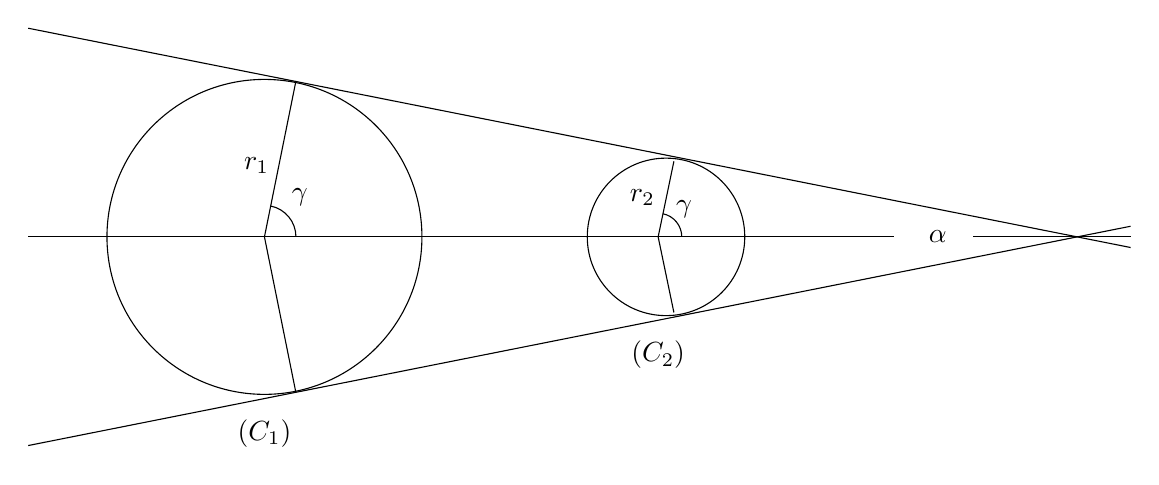
\begin{tikzpicture}

  \tkzDefPoints{0/0/A, 0.4/1.98/B, 5/0/C, 5.2/0.96/D}

  \draw (0,0) circle (2);
  \draw (5.1,0) circle (1);

  % Tangent lines
  \draw (-3,-2.65) -- (11,0.135);
  \draw (-3,2.65) -- (11,-0.135);

  \draw (0, 0) -- (0.4, 1.98);
  \draw (0, 0) -- (0.4, -1.98);

  \draw (5, 0) -- (5.2, 0.96);
  \draw (5, 0) -- (5.2, -0.96);

  \draw (-3, 0) -- (8, 0);
  \draw (9,0) -- (11,0);

  \tkzMarkAngle[size=0.4](C,A,B)
  \tkzMarkAngle[size=0.3, xshift=5cm, yshift=0cm](C,A,B)

  \node at (0,-2.5) {$(C_1)$};
  \node at (5,-1.5) {$(C_2)$};
  \node at (-0.1, 0.91) {$r_{1}$};
  \node at (0.45, 0.5) {$\gamma$};
  \node at (4.8, 0.5) {$r_{2}$};
  \node at (5.33, 0.35) {$\gamma$};
  \node at (8.55,0) {$\alpha$};

\end{tikzpicture}
\end{document}

\end{center}

\begin{proof}
  Let's focus on the triangle created by the tagent lines to those circles :

  \begin{center}
    \documentclass[tikz,border=2pt]{standalone}
\usepackage{tkz-euclide}
\usepackage{amsmath}

\begin{document}

\begin{tikzpicture}[scale=1.2]

  % --- Points ---
  \coordinate (A) at (0,0);
  \coordinate (B) at (0,4);
  \coordinate (C) at (3,0);
  \coordinate (D) at (3,2.5);
  \coordinate (E) at (8,0);

  % --- Base line ---
  \draw (0,0) -- (8,0);

  % --- Vertical radii ---
  \draw (A) -- (B);
  \draw (C) -- (D);

  % --- Tangent line ---
  \draw[thick] (B) -- (E);

  % --- Right angle marks ---
  \draw (0,0) rectangle (0.35,0.35);
  \draw (3,0) rectangle (3.35,0.35);

  % --- Angle gamma left ---
  \draw (B) ++(270:0.6) arc (270:330:0.6);
  \node at (0.4,3.1) {$\gamma$};

  % --- Angle gamma right ---
  \draw (D) ++(270:0.5) arc (270:330:0.5);
  \node at (3.4,1.8) {$\gamma$};

  % --- Angle alpha ---
  \draw (E) ++(145:0.5) arc (130:222:0.25);
  \node at (6.7,0.29) {$\dfrac{\alpha}{2}$};

  % --- Labels ---
  \node[left]  at ($(A)!0.5!(B)$) {$r_1$};
  \node[right] at ($(C)!0.5!(D)$) {$r_2$};

  \node at (1.9,3.5) {$d$};
  \node at (5.9,1.5) {$d'$};

\end{tikzpicture}

\end{document}

  \end{center}
\end{proof}

\end{document}
